\documentclass[a4paper]{article}
\usepackage{vntex}
%\usepackage[english,vietnam]{babel}
%\usepackage[utf8]{inputenc}

%\usepackage[utf8]{inputenc}
%\usepackage[francais]{babel}
\usepackage{a4wide,amssymb,epsfig,latexsym,multicol,array,hhline,fancyhdr}

\usepackage{amsmath}
\usepackage{lastpage}
\usepackage[lined,boxed,commentsnumbered]{algorithm2e}
\usepackage{enumerate}
\usepackage{listings}
\usepackage{color}
\usepackage{graphicx}							% Standard graphics package
\usepackage{array}
\usepackage{tabularx, caption}
\usepackage{subcaption}
\usepackage{multirow}
\usepackage{multicol}
\usepackage{rotating}
\usepackage{graphics}
\usepackage{geometry}
\usepackage{setspace}
\usepackage{epsfig}
\usepackage{tikz}
\usetikzlibrary{arrows,snakes,backgrounds}
\usepackage{hyperref}
\hypersetup{urlcolor=blue,linkcolor=black,citecolor=black,colorlinks=true} 
%\usepackage{pstcol} 								% PSTricks with the standard color package

\newtheorem{theorem}{{\bf Định lý}}
\newtheorem{property}{{\bf Tính chất}}
\newtheorem{proposition}{{\bf Mệnh đề}}
\newtheorem{corollary}[proposition]{{\bf Hệ quả}}
\newtheorem{lemma}[proposition]{{\bf Bổ đề}}


%\usepackage{fancyhdr}
\setlength{\headheight}{40pt}
\pagestyle{fancy}
\fancyhead{} % clear all header fields
\fancyhead[L]{
 \begin{tabular}{rl}
    \begin{picture}(25,15)(0,0)
    \put(0,-8){
\includegraphics[width=8mm, height=8mm]{hcmut.png}}
    %\put(0,-8){\epsfig{width=10mm,figure=hcmut.eps}}
   \end{picture}&
	%
\includegraphics[width=8mm, height=8mm]{hcmut.png} & %
	\begin{tabular}{l}
		\textbf{\bf \ttfamily Trường Đại Học Bách Khoa Tp.Hồ Chí Minh}\\
		\textbf{\bf \ttfamily Khoa Khoa Học và Kỹ Thuật Máy Tính}
	\end{tabular} 	
 \end{tabular}
}
\fancyhead[R]{
	\begin{tabular}{l}
		\tiny \bf \\
		\tiny \bf 
	\end{tabular}  }
\fancyfoot{} % clear all footer fields
\fancyfoot[L]{\scriptsize \ttfamily Bài tập lớn môn Mật mã và an minh mạng - Niên khóa 2018-2019}
\fancyfoot[R]{\scriptsize \ttfamily Trang {\thepage}/\pageref{LastPage}}
\renewcommand{\headrulewidth}{0.3pt}
\renewcommand{\footrulewidth}{0.3pt}


%%%
\setcounter{secnumdepth}{4}
\setcounter{tocdepth}{3}
\makeatletter
\newcounter {subsubsubsection}[subsubsection]
\renewcommand\thesubsubsubsection{\thesubsubsection .\@alph\c@subsubsubsection}
\newcommand\subsubsubsection{\@startsection{subsubsubsection}{4}{\z@}%
                                     {-3.25ex\@plus -1ex \@minus -.2ex}%
                                     {1.5ex \@plus .2ex}%
                                     {\normalfont\normalsize\bfseries}}
\newcommand*\l@subsubsubsection{\@dottedtocline{3}{10.0em}{4.1em}}
\newcommand*{\subsubsubsectionmark}[1]{}
\makeatother


\begin{document}

\begin{titlepage}
\begin{center}
ĐẠI HỌC QUỐC GIA THÀNH PHỐ HỒ CHÍ MINH \\
TRƯỜNG ĐẠI HỌC BÁCH KHOA \\
KHOA KHOA HỌC - KỸ THUẬT MÁY TÍNH 
\end{center}

\vspace{1cm}

\begin{figure}[htp]
\begin{center}

\includegraphics[width=3cm]{hcmut.png}
\end{center}
\end{figure}

\vspace{1cm}


\begin{center}
\begin{tabular}{c}
\multicolumn{1}{l}{\textbf{{\Large Mật mã và an ninh mạng}}}\\
~~\\
\hline
\\
\multicolumn{1}{l}{\textbf{{\Large Đề tài}}}\\
\\
\textbf{{\Huge Ứng ụng mã hóa dữ liệu}}\\
\\
\hline
\end{tabular}
\end{center}

\vspace{3cm}

\begin{table}[h]
\begin{tabular}{rrl}
\hspace{5 cm} & GVHD: & Nguyễn Trần Hữu Nguyên\\
& SV: & Nguyễn Trần Lê Minh - 1511003 \\
& & Lê Duy Thanh - 1512990 \\
& & Nguyễn Xuân Nam - 1512098\\
\end{tabular}
\end{table}

\begin{center}
{\footnotesize TP. HỒ CHÍ MINH, THÁNG 03/2019}
\end{center}
\end{titlepage}


%\thispagestyle{empty}

\newpage
\tableofcontents
\newpage

Mã hóa là phương pháp bảo vệ dữ liệu cá nhân nhạy cảm trên máy tính của bạn. Việc mã hóa còn ngăn chặn bất cứ ai đọc dữ liệu của bạn khi bạn gửi thông tin qua mạng hay đồng bộ lên máy chủ, cloud,...\\

Trong bài tập lớn này, nhóm sẽ thực hiện một số giải thuật mã hóa dễ cho các tập tin trong máy được an toàn.

%%%%%%%%%%%%%%%%%%%%%%%%%%%%%%%%%
\section{Giới thiệu đề tài}
Nhóm đã hiện thực ba giải thuật mã hóa phổ biến đó là RSA, DES và Steganography.\\

Với RSA và DES, nhóm đọc dữ liệu cần mã hóa (plaint text) từ tệp văn bản (*.txt file - text file). Đối với Steganography, nhóm đọc dữ liệu từ text file trộn vào một ảnh mang.
Để chứng minh plaint text trùng với dữ liệu được giải mã, nhóm sử dụng hàm băm để đối chiếu hai tệp.

%%%%%%%%%%%%%%%%%%%%%%%%%%%%%%%%%
\section{Cấu trúc của ứng dụng}
%TODO: mỗi thiết bị như gateway, mobile phải có kiến trúc tổ chức trong này
Cấu trúc của ứng dụng được miêu tả trong hình \ref{fig:file_structure}:
\begin{figure}[htp]
    \centering
    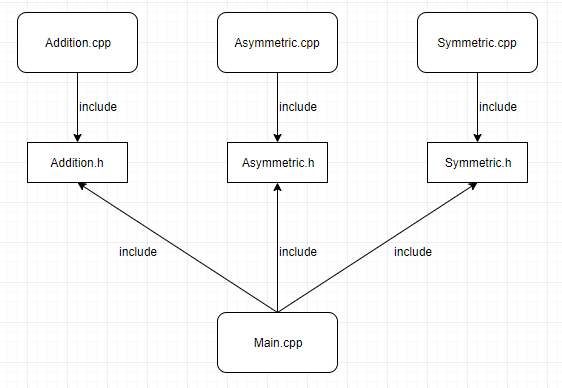
\includegraphics[scale=1]{file_structure.png}
    \caption{Kiến trúc chính của hệ thống}
    \label{fig:file_structure}
\end{figure}
Chương trình gồm 4 mô đun chính là:
\begin{itemize}
    \item Symmetric: Chứa các hàm mã hóa tập tin sử dụng giải thuật DES.
    \item Asymmetric: Chứa các hàm mã hóa tập tin sử dụng giải thuật RSA.
    \item Addition: Chứa các hàm mã hóa tập tin sử dụng kỹ thuật giấu tin (Steganography).
    \item Main: Đọc các đối số và gọi các hàm phù hợp trong ba thư viện trên.
\end{itemize}
	\subsection{Mạng cảm biến}
	...
	
	\subsection{Server}
	Các tệp tin và các trang ở server được tổ chức như sau:
	\begin{figure}[htp]
	    \centering
	    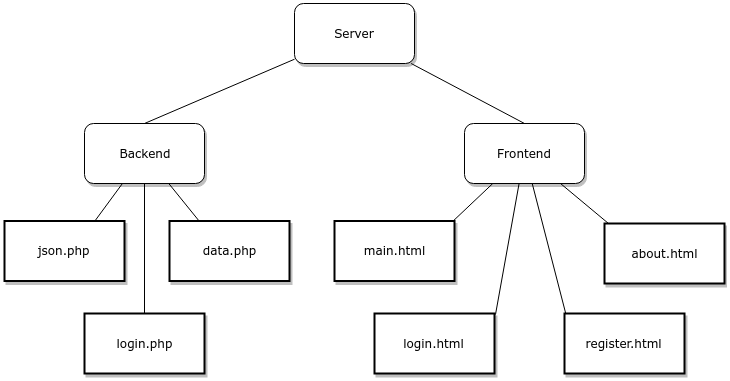
\includegraphics[scale=0.5]{serverStructure.png}
	    \caption{Kiến trúc tệp tin tại server}
	    \label{fig:my_label}
	\end{figure}
	Các trang tại server phục vụ cho các yêu cầu của đề tài:
	    \subsubsection{Backend}
	        \begin{itemize}
	            \item json.php: trả về dữ liệu dưới dạng JSON. Dữ liệu này được các cảm biến gửi lên và chứa trong cơ sở dữ liệu.
	           \item data.php: nơi các gateway sẽ gửi dữ liệu được tổng hợp từ các sensor. Dữ liệu này sau đó sẽ được đưa vào cơ sở dữ liệu.
	           \item login.php: xử lí các đăng kí và đăng nhập từ người dùng.
	        \end{itemize}
	   \subsubsection{Frontend}
	        \begin{itemize}
	            \item main.html: trang chính của người dùng, cung cấp việc lựa chọn các gateway đang có dữ liệu và vẽ biểu đồ theo thời gian.
	            \item about.html: các thông tin về nhóm phát triển và đề tài.
	            \item register.html: trang chưa thông tin đăng kí bởi người dùng.
	            \item login.html: trang đăng nhập để vào ứng dụng.
	        \end{itemize}
%%%%%%%%%%%%%%%%%%%%%%%%%%%%%%%%%
	\subsection{Ứng dụng di động}
		\subsubsection{Android}
		\begin{enumerate}
		\item \textbf{ Sơ đồ trạng thái của ứng dụng.}\\
			Với dứng dụng android, phần mềm được thực thi bằng các activity ứng với mỗi nhiệm vụ khác nhau. Trong bái tập lớn 			này, nhóm sử dụng các activity cơ bản sau:
 			\begin{itemize} 
				\item Đăng nhập (MainActivity hay LoginActivity), 
				\item Danh sách dữ liệu thô (HomeActivity),
				\item Biểu đồ đường (LineChartActivity),
				\item Biểu đồ phân bố (DistributionChartActivity).
			\end{itemize} 
			Các activity giao tiếp với nhau thông qua intent của android theo sơ đồ hình \ref{fig:sateDiagramApp}:\\
			\begin{figure}[htp]
	    			\centering
	   			 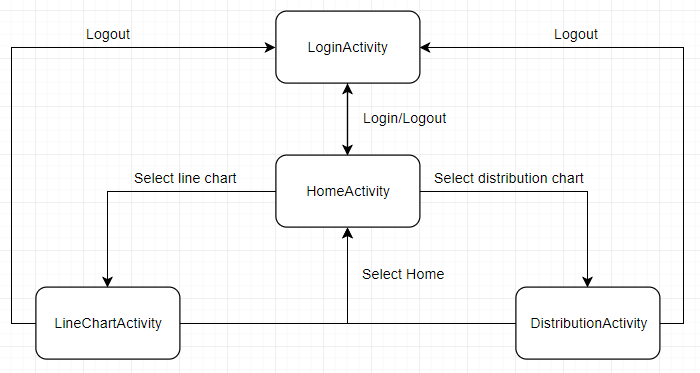
\includegraphics[scale=0.75]{StateDiagramApp.PNG}
	   			 \caption{Sơ đồ chuyển trạng thái của các activity}
	   			 \label{fig:sateDiagramApp}
			\end{figure}\\
			\textbf{LoginActivity} là hoạt động đầu tiên khi bắt dầu sử dụng ứng dụng.\\
			\textbf{HomeActivity} quản lí một danh sách các dữ liệu thô lấy từ server. Danh sách này chỉ trỏ đến một nốt cụ thể 				(bao gồm một gatewayID và một nodeId) và chứa thông tin trong này ngày (tính từ 0 giờ). Vì dữ liệu có thể quá dài 				nên nhóm quyết định đặt gới hạn danh sách dài chỉ 20 phần tử.\\	
			\textbf{LineChartActivity}: Giống HomeActivity, hoạt động này cũng lấy một mảng các gateway từ server. Tuy 					nhiên, dữ liệu lấy về được vẽ thành biểu đồ đường thể thấy trực quan sự biển đổi theo thời gian. Và gới hạn của các 				điễm vẽ biểu đồ cũng là 20 giống HomeActivity.\\
			\textbf{DistributionChartActivity}: Các activity đều lấy dữ liệu từ server về. Với hoạt động này. Các dữ liệu lấy về sẽ 			được chia thành 10 nhóm tương ứng với 0-9,10-19,...90-100. Số lượng phần tử trong mỗi nhóm sẽ là căn cứ để tính 				ra phần trăm đóng góp của môi nhóm trong toàn một dữ iệu lấy về được. Từ đó là vẽ được biểu đồ phân bố giá trị.\\
		\item \textbf{Cấu trúc dữ liệu của ứng dụng.}\\
			Cấu trúc dữ liệu của ứng dụng được tổ chức theo cấu trúc của tệp json lấy từ server và được thể hiện thông qua 				sơ đồ hình \ref{fig:dataStructureApp}.
			\begin{figure}[htp]
	    			\centering
	   			 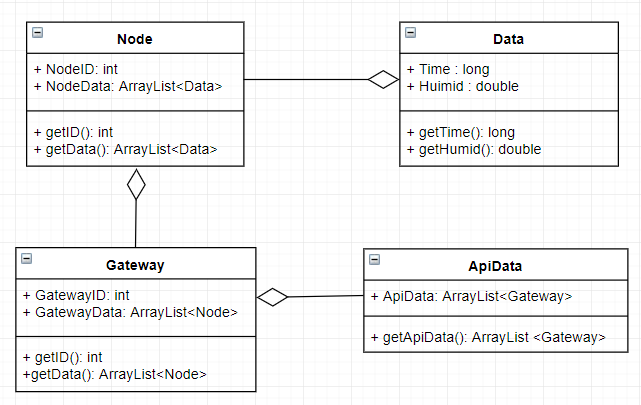
\includegraphics[scale=0.5]{DataStructure.PNG}
	   			 \caption{Cấu trúc dữ liệu của ứng dụng}
	   			 \label{fig:dataStructureApp}
			\end{figure}\\
			 \textbf{Data} là lớp chứa dữ liệu mà một cảm biến gửi cho gateway tại một thời điểm. Vì vậy lớp này gồm 2 thuộc 				tính là thời gian (time) và độ ẩm (huminity).\\
			 \textbf{Node} là đơn vị quản lí dữ liệu của một cảm biến. Nó gồm định danh của cảm biến và một mảng các giá trị mà 			cảm biến thu nhận được.\\
			 \textbf{Gateway}: Một gateway quản lí nhiều cảm biến bởi vậy nó cần chứa một mảng các cảm biến (bao gồm định 
			danh và dữ liệu của chúng). Đồng thời mỗi gateway cũng có định danh riêng của chúng.\\
			 \textbf{ApiData} là dữ liệu nơi lưu trữ dữ liệu lấy được tệp json. Nó gôm một mảng các gateway.\\
		\item \textbf{Lấy dữ liệu từ tệp json}.\\
			Lấy dữ liệu từ server là một phần quan trọng của ứng dụng. Việc này được quản lí bới ApiController với cấu trúc hình 				 \ref{fig:ApiGetDataDiagramApp}:\\
			\begin{figure}[htp]
	    			\centering
	   			 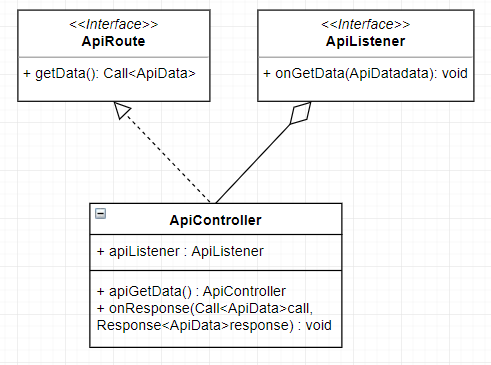
\includegraphics[scale=0.75]{ApiGetDataDiagram.PNG}
	   			 \caption{Cấu trúc của ApiController}
	   			 \label{fig:ApiGetDataDiagramApp}
			\end{figure}\\
			\textbf{ApiController} chứa các phần tử sau:
			\begin{itemize} 
				\item Đường dẫn đến địa chỉ chứa tệp json. Ví dụ: \\
				\begin{lstlisting}[language=Java]
public static final String BASE_URL = "http://10.20.83.74/backend/";
				\end{lstlisting}
				\item Sử dụng thư viện retrofit2 hiện thực phương thức getData() và trong constructure và trả dữ liệu về 						phương thức onRespone. 
			\end{itemize} 
			\textbf{ApiRoute} bao gồm địa chỉ của tệp json và phương thức getData().\\
			\textbf{ApiListener} chứa phương thức onGetData sử lí dữ liệu lấy được từ json và được hiện thực trong các 					activity.
		\end{enumerate}

%%%%%%%%%%%%%%%%%%%%%%%%%%%%%%%%%
\section{Các giao thức sử dụng}
% TODO:
% mobile-web : giao thuc http
% gateway : stop and wait protocol
	\subsection{Hypertext Transfer Protocol}
    Hypertext Transfer Protocol(HTTP)\cite{HTTP} là một giao thức dùng trong việc truyền các dữ liệu trên các web. Là một phương thức sử dụng mô hình client-server. Server sẽ lắng nghe ở cổng 80 và trả lời các yêu cầu từ client. Dữ liệu trả về từ server bao gồm các mã trạng thái (status code) để  cho biết tình trạng truy cập của người dùng. Các mã trạng thái thường gặp như 200 -thành công, 301- chuyển trang, 404- trang không tìm thấy....\\
    
    HTTP cung cấp nhiều phương thức cho người sử dụng nhưng có 2 phương thức được sử dụng chính trong bài tập lớn của nhóm:
    \begin{itemize}
        \item POST: đây là phương thức dùng để  gửi dữ liệu từ gateway lên server. POST cho phép gửi kèm dữ liệu từ client tới server trong gói tin.
        \item GET: đây là phương thức dùng để lấy dữ liệu từ server mà trong bài tập lớn này là dữ liệu JSON từ server.
    \end{itemize}
	
	
	\subsection{Stop and Wait}
	...
%%%%%%%%%%%%%%%%%%%%%%%%%%%%%%%%%
\section{Các tính năng của hệ thống}
Hệ thống đáp ứng được các yêu cầu cơ bản của một hệ thống theo dõi độ ẩm đất bao gồm:
\begin{itemize}
    \item Thu thập dữ liệu về độ ẩm đất từ các cảm biến.
    \item Vẽ biểu đồ cho thấy sự biến động về độ ẩm trong ngày.
    \item Có khả năng kiểm tra các thông báo về nhiệt độ và lượng mưa của khu vực bằng các opensource API\cite{weatherAPI}.
    \item Hệ thống có sự quản lí phân cấp và có khả năng mở rộng.
\end{itemize}
%%%%%%%%%%%%%%%%%%%%%%%%%%%%%%%%%
\section{Hướng dẫn vận hành}
% TODO:
% mobile : hướng dẫn sử dụng và các thành phần trên giao diện
% gateway : hướng dẫn setup gateway và gửi dữ liệu tới server
% server: Setup server và sử dụng website
	\subsection{Cách cài đặt server}
	
    Để có thể cài đặt và sử dụng localhost, chúng ta cần cài đặt một phần mềm có khả năng lắng nghe cổng 80 của máy tính. Ở đây nhóm sử dụng phần mềm xampp là một phần mềm miễn phí bao gồm :
    \begin{itemize}
        \item Apache: cho phép lắng nghe cổng 80 để tiếp nhận các yêu cầu.
        \item Mysql: đây là cơ sở dữ liệu có cấu trúc miễn phí.
        \item PHP: là một ngôn ngữ rất phổ biến được sử dụng ở server.
    \end{itemize}
    
    Phần mềm có thể tải về tại đường dẫn: \url{https://www.apachefriends.org/index.html}.\\
    
    Sau khi cài đặt xampp, chúng ta có thể sử dụng mạng wifi hoặc tự phát wifi. \\
    
    Kế tiếp, để có thể gửi dữ liệu từ client lên server ta cần sửa lại địa chỉ của server (mặc định là 127.0.0.1) thành địa chỉ trong mạng LAN bằng cách sửa file \textit{httpd.conf} tại đường dẫn \textit{etc/httpd.conf}\\
    
    \lstinline{51 Listen <your local ip address>}\\
    
    Tải toàn bộ mã nguồn tại: \url{https://github.com/lochoang75/IoT_Lab}\\
    
    Khởi chạy xampp và vào đường dẫn \url{http://localhost/phpmyadmin} để 
    nhập cơ sở dữ liệu.
    
    \begin{figure}[htp]
        \centering
        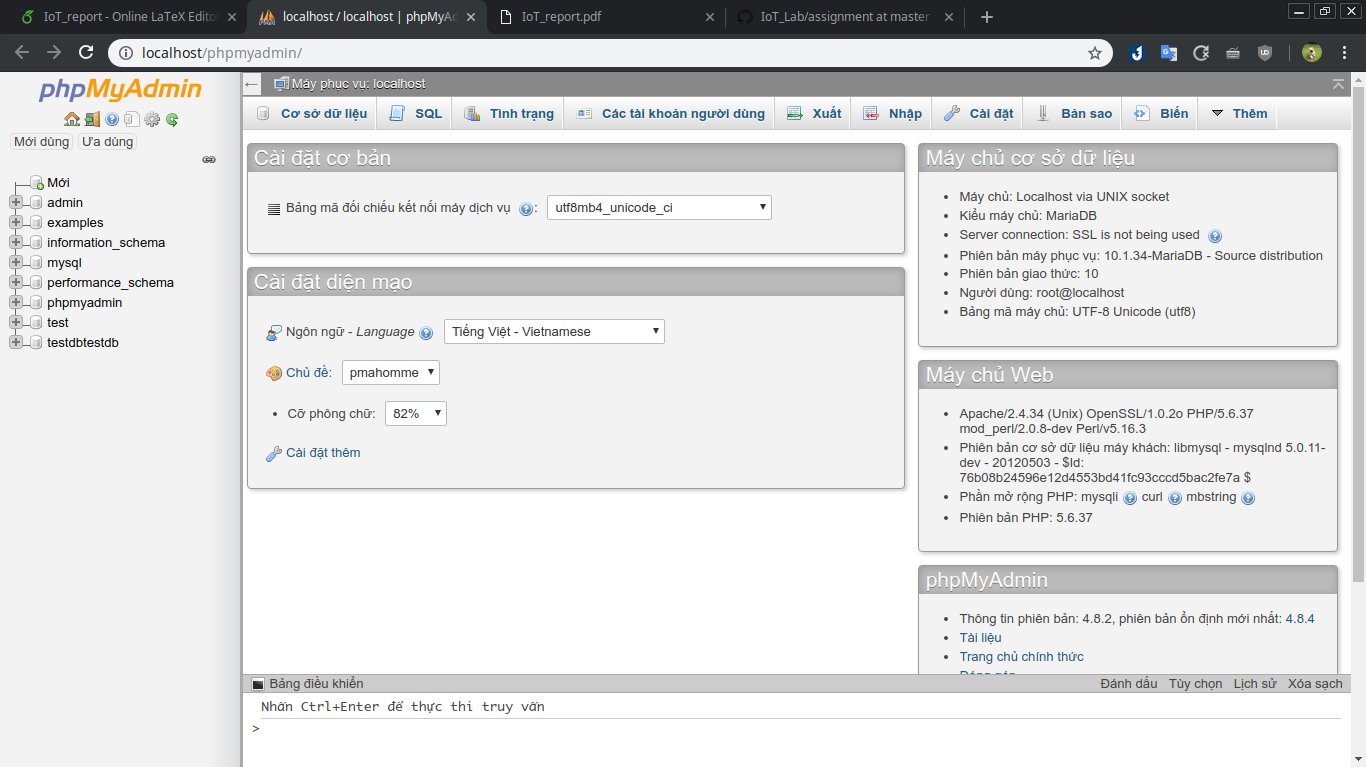
\includegraphics[scale=0.3]{phpmyadmin.png}
        \caption{Giao diện phpmyadmin}
        \label{fig:my_label}
    \end{figure}
    Tạo một bảng có tên test và chọn vào \textbf{nhập(import)}, chọn file \textit{test.sql} để chèn cơ sở dữ liệu bao gồm 2 bảng như hình bên dưới.
    \begin{figure}[htp]
        \centering
        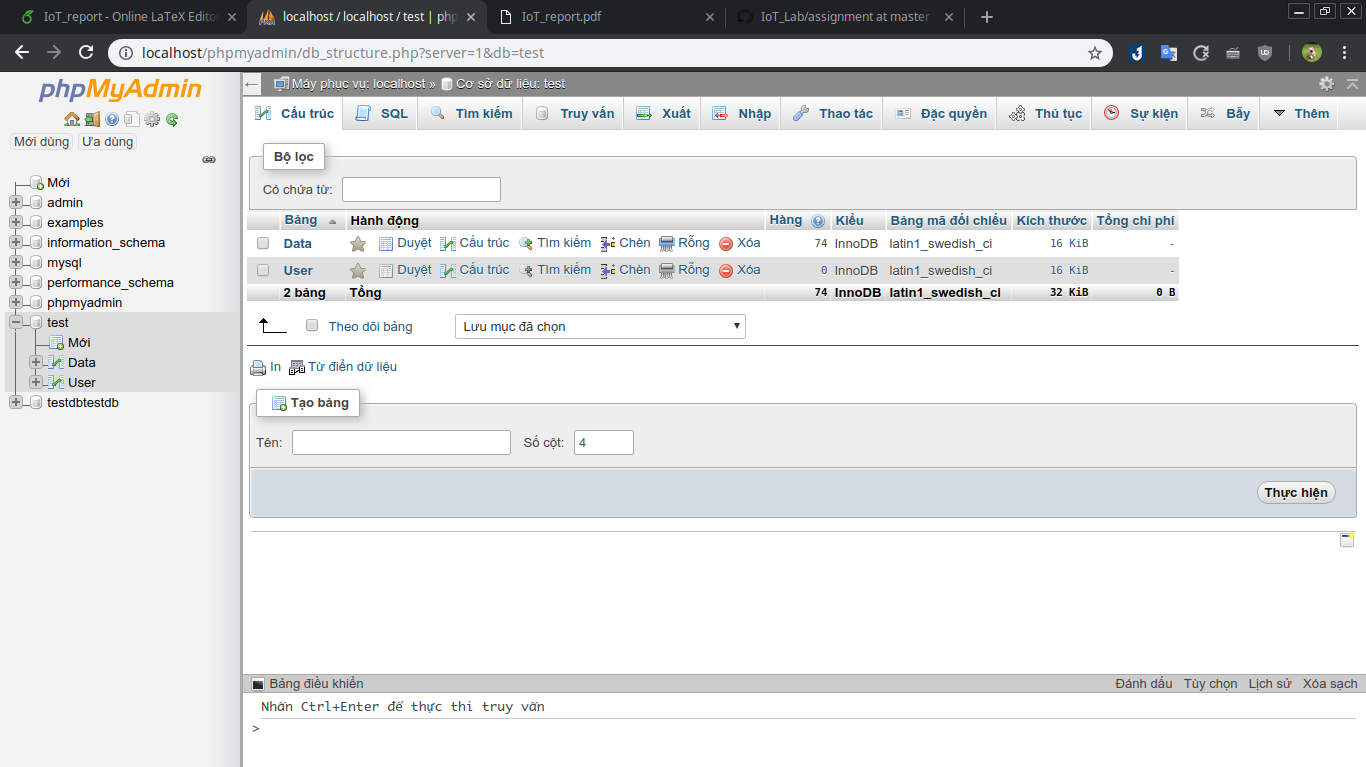
\includegraphics[scale=0.3]{database.png}
        \caption{Kết quả sau khi nhập thành công database}
        \label{fig:my_label}
    \end{figure}
    
    Cuối cùng chuyển thư mục backend và frontend vào thư mục htdocs(thư mục root mặc định của localhost). Nếu thành công các đường dẫn cho các file ở server sẽ là:
    \begin{itemize}
        \item about.html: \url{http://localhost/frontend/about.html}
        \item main.html: \url{http://localhost/frontend/main.html}
        \item register.html: \url{http://localhost/frontend/register.html}
        \item login.html:
        \url{http://localhost/frontend/login.html}
        \item json.php: \url{http://localhost/backend/json.php}
        \item data.php: \url{http://localhost/backend/data.php}
        \item login.php: \url{http://localhost/backend/login.php}
    \end{itemize}
    \subsection{Sử dụng các tính năng của website}
    Sau khi cài đặt xong server, trang chính sẽ như hình sau:
    \begin{figure}[htp]
        \centering
        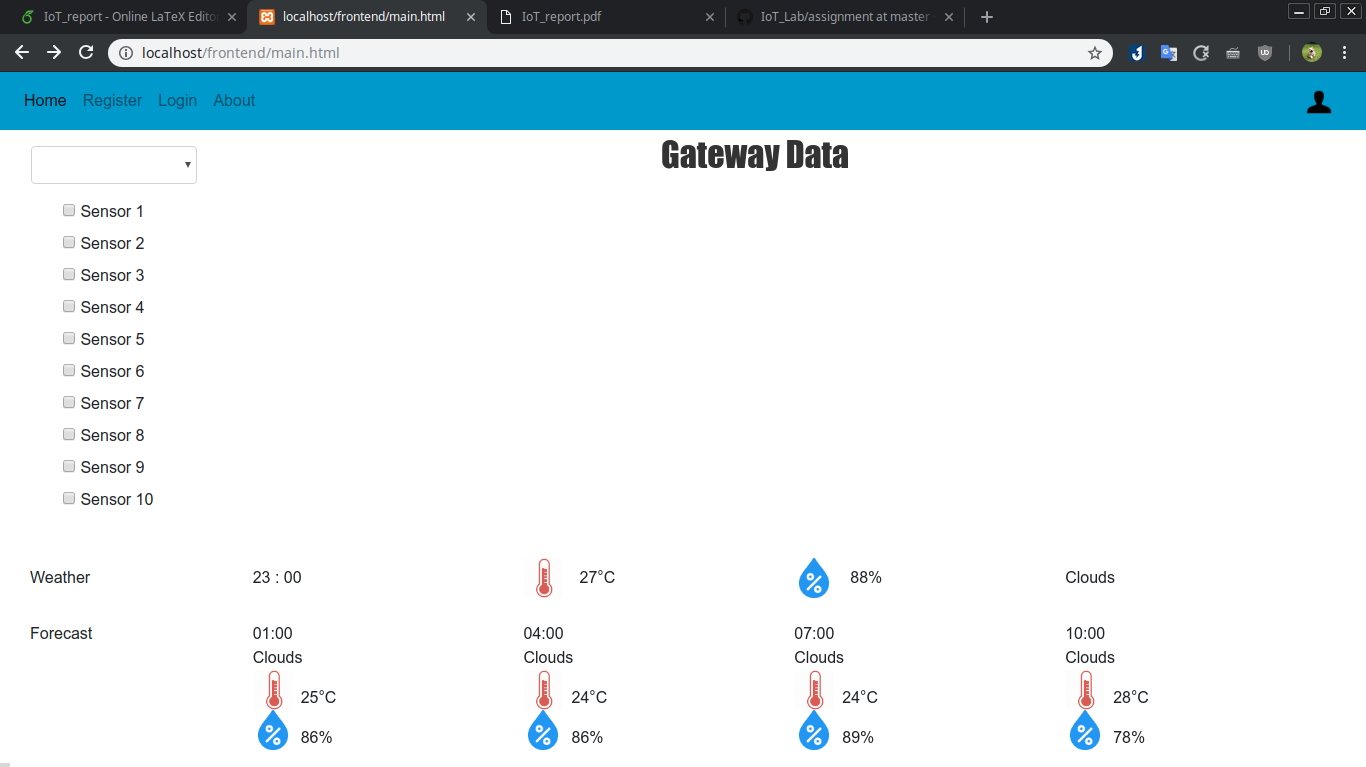
\includegraphics[scale=0.3]{mainpage.png}
        \caption{Giao diện trang chính}
        \label{fig:my_label}
    \end{figure}
    
    Để hiển thị được biểu đồ, người dùng cần chọn gateway cần hiển thị. Các cảm biến có dữ liệu sẽ cho phép chọn:
    \begin{figure}[htp]
        \centering
        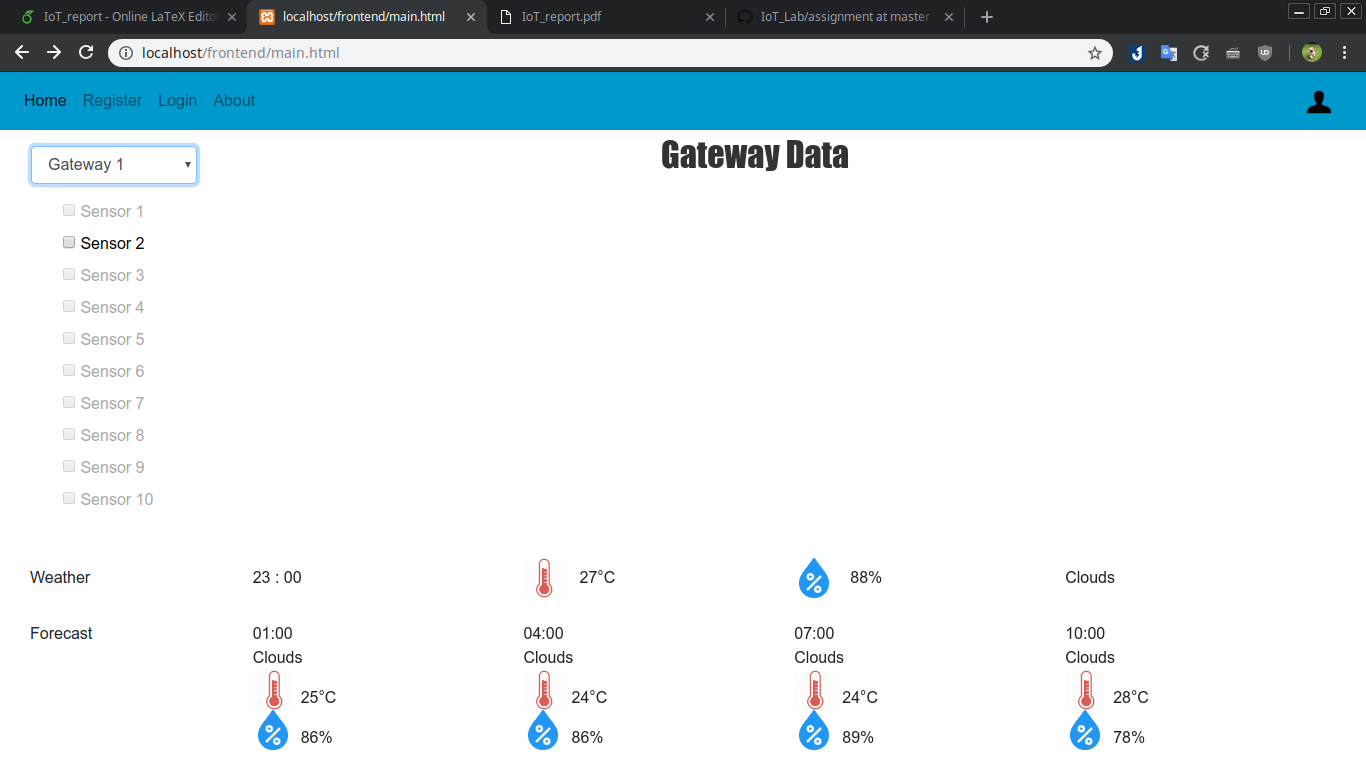
\includegraphics[scale=0.3]{gatewaySelect.png}
        \caption{Giao diện sau khi chọn gateway}
        \label{fig:my_label}
    \end{figure}
    Cuối cùng chọn một hoặc một vài cảm biến và đồ thị của cảm biến đó sẽ được vẽ ra.
    \begin{figure}[htp]
        \centering
        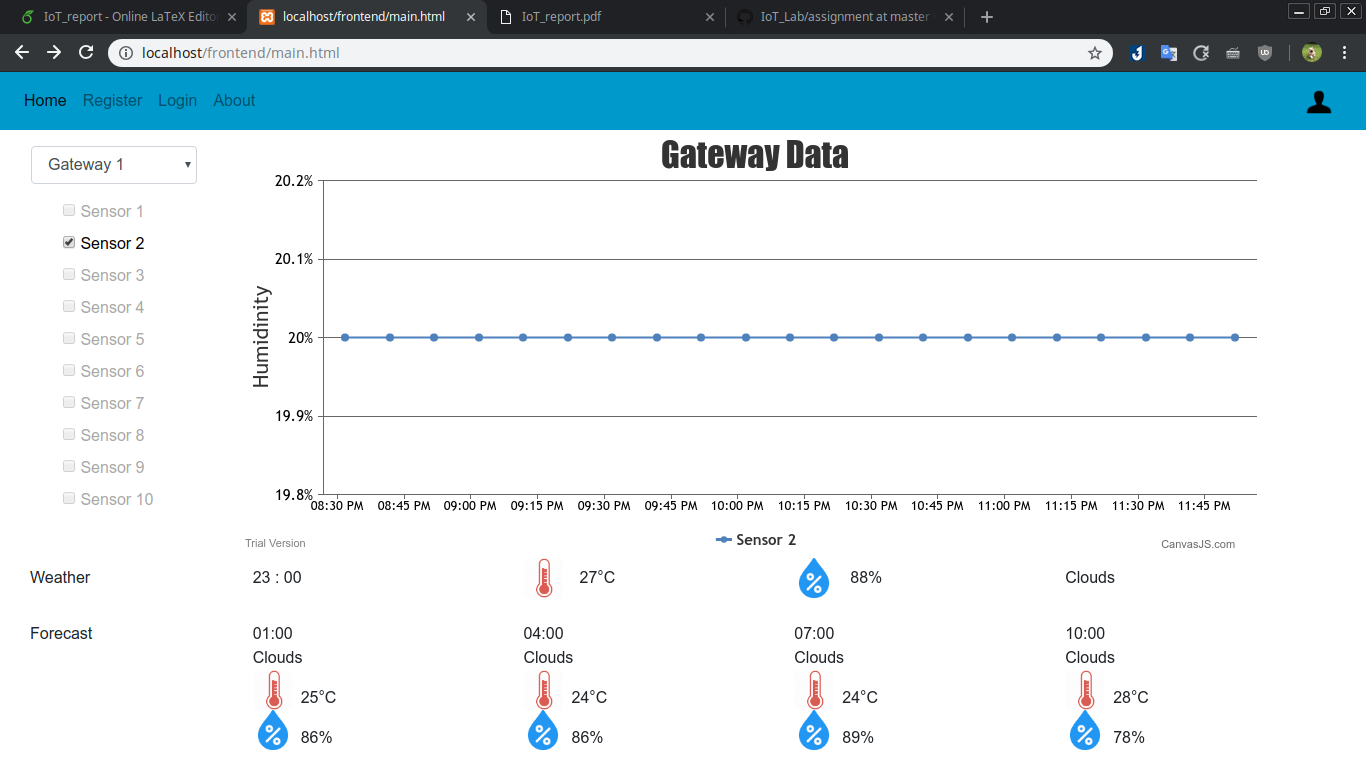
\includegraphics[scale=0.3]{sensorSelect.png}
        \caption{Giao diện sau khi chọn gateway}
        \label{fig:my_label}
    \end{figure}
    Phần dưới của website là các thông tin dự báo về nhiệt độ và độ ẩm theo từng thời điểm trong ngày và được cập nhật mỗi giờ.
    

%%%%%%%%%%%%%%%%%%%%%%%%%%%%%%%%%
	\subsection{Sử dụng ứng di động}
	\subsubsection{Android}
	Bước đầu tiên để sử dụng ứng dụng là cài đặt. Sử dụng android studio chạy mã nguồn từ địa chỉ \url{https://github.com/lochoang75/IoT_Lab/tree/master/assignment/iotapp}.\\
	Sau khi cài đặt, mở ứng dụng ta thấy màn hình đăng nhập như hình \ref{fig:LoginActivityApp}\\
	\begin{enumerate}
	\item \textbf{Màn hình đăng nhập}\\
	\begin{figure}[htp]
       		\centering
       		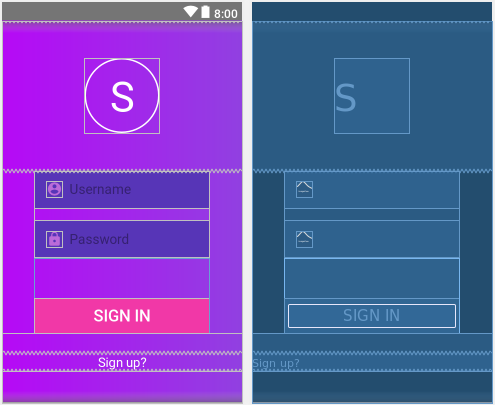
\includegraphics[scale=0.5]{LoginActivity.png}
        		\caption{Giao diện sau khi chọn gateway}
       		 \label{fig:LoginActivityApp}
    	\end{figure}\\
	Chọn đăng nhập chúng ta chuyển đến màn hình chính của ứng dụng như hình \ref{fig:DefaultHomeApp}.\\
	
	\item \textbf{Màn hình chính}\\
	\begin{figure}[!tbp]
\centering
  \begin{subfigure}[b]{0.3\textwidth}
    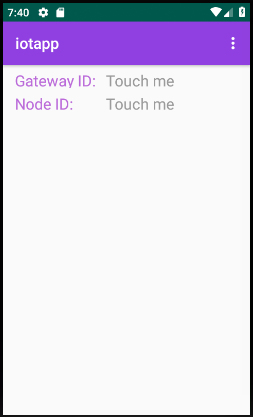
\includegraphics[width=\textwidth]{DefaultHome.png}
    \caption{Khởi tạo}
    \label{fig:DefaultHomeApp}
  \end{subfigure}
  \begin{subfigure}[b]{0.3\textwidth}
    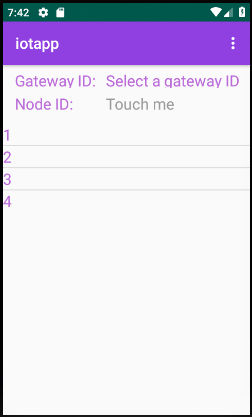
\includegraphics[width=\textwidth]{SelectgatewayID.png}
    \caption{Chọn gatewayID}
    \label{fig:SelectgatewayIDApp}
  \end{subfigure}
  \begin{subfigure}[b]{0.3\textwidth}
    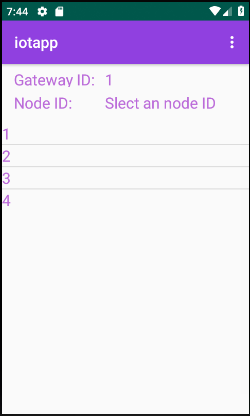
\includegraphics[width=\textwidth]{SelectnodeID.png}
    \caption{Chọn nodeID}
    \label{fig:SelectnodeIDApp}
  \end{subfigure}
  \caption{Màn hình chính}
 \end{figure}\\
	Tại một thời điểm chỉ có thông tin của một cảm biến được hiển thị, vì thế chúng ta cần chọn định danh cho nó (bao gồm gatewayID 	và nodeId). Chạm vào "Touch me" để chọn các thông tin tương ứng. Lưu ý: NodeId chỉ được chọn khi gatewayId hợp lệ (đã được 	chọn).\\
	Sau khi chọn xong định danh, trên màn hình sẽ hiển thị một danh sách thông tin thu thập được từ cảm biến như hình \ref{fig:listviewHomeApp}. Để tải lại dữ liệu, người dùng có thể lướt màn hình từ trên xuống.\\

	\begin{figure}[htp]
		  \centering
 		 \begin{minipage}[b]{0.3\textwidth}
   			 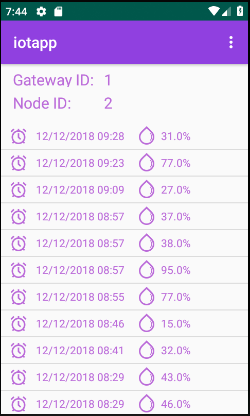
\includegraphics[width=\textwidth]{listviewHome.png}
   			 \caption{Danh sách dữ liệu}
			\label{fig:listviewHomeApp}
  		\end{minipage}
 		 \hfill
 		 \begin{minipage}[b]{0.3\textwidth}
   			 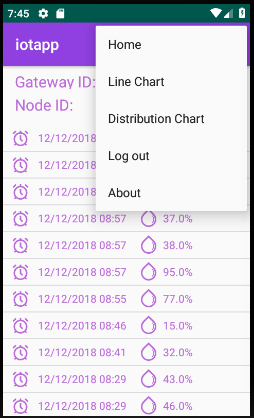
\includegraphics[width=\textwidth]{MenuApp.png}
   			 \caption{Menu của ứng dụng}
			 \label{fig:MenuApp}
 		 \end{minipage}
	\end{figure}
	Trên góc trên bên phải màn hình có nút menu. Chọn menu để chuyển tới các màn hình khác. Khi chọn menu, chúng ta thấy xuất 		hiện hình \ref{fig:MenuApp}\\
	\item \textbf{Menu}\\
	Menu bao gồm các phần sau:\\
		\begin{itemize}
		\item \textbf{Home} Chuyển đến màn hình chính.\\
		\item \textbf{Line Chart} Chuyển đến màn hình biểu đồ đường (xem mục \ref{linechartsection})\\
		\item \textbf{Distribution Chart} Chuyển đến màn hình biểu đồ phân b.(xem mục \ref{distributionchartsection})\\
		\item \textbf{Logout} Chuyển đến màn hình đăng nhập.
		\end{itemize}	
	\item \textbf{Màn hình biểu đồ đường} \label{linechartsection}\\
	\begin{figure}[htp]
       		\centering
       		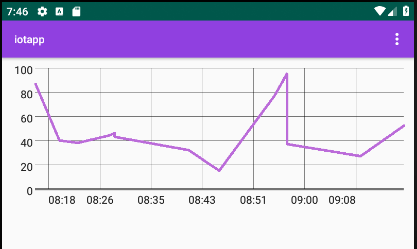
\includegraphics[scale=0.7]{linechart.png}
        		\caption{Biểu đồ đường}
       		 \label{fig:linechartApp}
    	\end{figure}\\
	Dữ liệu từ màn hình chính sẽ được vễ thành biểu đồ tại đây. Lưu ý: chỉ có thể chuyển đế màn hình này khi định danh của cảm 			cảm biến đã được chọn.\\
	Trục X là trục thời gian từ 0 giờ đến 24 giờ.\\
	Trục Y là trục giá trị độ ẩm từ 0 đến 100 phần trăm.
	\item \textbf{Màn hình biểu đồ phân bố}\label{distributionchartsection}\\
	\begin{figure}[htp]
       		\centering
       		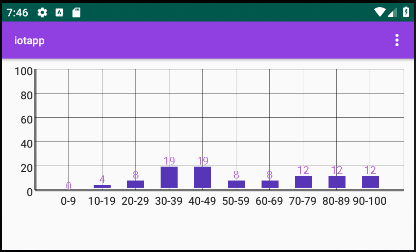
\includegraphics[scale=0.7]{distributionchart.png}
        		\caption{Biểu đồ phân bố}
       		 \label{fig:distributionchartApp}
    	\end{figure}\\
	Dữ liệu từ tệp json sẽ được tính ra phần trăm đóng góp của các nhóm và được biểu thị trên biểu đồ.\\
	Trục X là trục của các nhóm tương ứng mới giá trị độ ẩm của mỗi data nhận được.\\
	Trục Y là giá trị phần trăm đóng góp của mỗi nhóm mà mỗi nhóm đóng góp.\\
	\end{enumerate}
%%%%%%%%%%%%%%%%%%%%%%%%%%%%%%%%%
\section{Kết luận}
	Kết luận về các nội dung và kết quả thực hiện được.


%%%%%%%%%%%%%%%%%%%%%%%%%%%%%%%%%
\begin{thebibliography}{80}


\bibitem{HTTP}
HTTP Definnition, \url{https://techterms.com/definition/http}


\bibitem{weatherAPI}
\url{https://openweathermap.org/api}


\end{thebibliography}
\end{document}

